\documentclass[12pt]{article}
\usepackage[margin=1in]{geometry}% Change the margins here if you wish.
\usepackage{amsmath,amsthm,amssymb,stmaryrd}
\usepackage[english]{babel}
\setlength{\parindent}{0pt} % This is the set the indent length for new paragraphs, change if you want.
\setlength{\parskip}{5pt} % This sets the distance between paragraphs, which will be used anytime you have a blank line in your LaTeX code.
\usepackage[textwidth=1.9cm,textsize=small]{todonotes}
\usepackage{hyperref}
\usepackage{tikz}
\usetikzlibrary{automata, positioning, arrows}
\tikzset{
    ->, % makes the edges directed
    >=stealth, % makes the arrow heads bold
    node distance=3cm, % specifies the minimum distance between two nodes. Change if necessary.
    every state/.style={thick, fill=gray!10}, % sets the properties for each ’state’ node
    initial text=$ $, % sets the text that appears on the start arrow
    }

\newcommand{\ifilip}[1]{\todo[inline,color=green!10]{{\bf Filip:} #1}}
\newcommand{\filip}[1]{\todo[color=green!10]{{\bf Filip:} #1}}

\newcommand{\iolek}[1]{\todo[inline,color=red!10]{{\bf Olek:} #1}}
\newcommand{\olek}[1]{\todo[color=red!10]{{\bf Olek:} #1}}


\newcommand{\icol}[1]{% inline column vector
  \left(\begin{smallmatrix}#1\end{smallmatrix}\right)%
}

\usepackage[capitalise]{cleveref}

\theoremstyle{definition}
\newtheorem{definition}{Definition}[section]
\newtheorem{theorem}{Theorem}[section]
\newtheorem{corollary}{Corollary}[section]
\newtheorem{fact}{Fact}[section]
\newtheorem{lemma}[theorem]{Lemma}
\newtheorem{example}{Example}[section]

\title{Sequences definable by 1-letter quantitative logics}
\author{Aleksander Wisniewski}
\date{\today}

\begin{document}
\maketitle

\section{Introduction}
It is an important result in computer science that the class of languages defined by finite automata coincides with the languages defined using MSO logic~\cite{Buchi1960}. Finite automata allow us to recognize languages, i.e., to accept or reject words over a given alphabet. Sch{\"{u}}tzenberger~\cite{Schutzenberger61b} extended the model of finite automata to make it possible to calculate quantitative properties of words. He introduced a model of weighted automata, which have richer semantics than finite automata. In weighted automata, transitions are supplied with weights (values from a semiring) and weights along a fixed run are multiplied using the semiring product. A value corresponding to a given input word is the semiring sum of values over all runs. Weighted automata calculate what we call a formal power series: a function from words to the semiring domain, $S: \Sigma^* \rightarrow K$.

Manfred Droste and Paul Gastin introduced a logic that coincides with weighted automata~\cite{DrosteG07}, in the same spirit as MSO logic coincides with finite automata. Their logic is called \emph{weighted logic}, and its semantics allows defining formal power series like weighted automata do. Unfortunately, the full ``natural'' form of weighted logic is richer than weighted automata, so the authors had to restrict the class of weighted logic expressions in order to capture the same expressiveness as weighted automata. The restrictions are both at the syntactic and semantic levels.

A follow up work on weighted logics is the work of Stephan Kreutzer and Cristian Riveros~\cite{KreutzerR13}. In their work, they introduced QMSO logic - Quantitative Monadic Second Order logic, which fulfills similar goals to the weighted logics of Manfred Droste and Paul Gastin but with easier definitions and a clearer distinction between the logical level (MSO) and the semiring level (addition/multiplication). They also had to restrict their logic to achieve the same power of expression as weighted automata, but their restriction is only at the syntactic level.

In this work, we explore the world of unrestricted QMSO expressions. More precisely, we will look into the properties of formal power series defined by unrestricted QMSO over a one-letter alphabet. Assume our alphabet is $\Sigma = \{a\}$. In this case words can be identified with their length. Thus the formal power series $S: \Sigma^* \rightarrow K$ can be seen as a sequence $S: \mathbb{N} \rightarrow K$, by mapping words $a^n$ to their length $n$. Restricted QMSO expressions coincide with weighted automata, and it is folklore that formal power series defined by weighted automata over a one-letter alphabet are exactly linear recursive sequences (see e.g.~\cite{BarloyFLM22}). It can be easily shown that sequences achieved using unrestricted QMSO form a richer class than linear recursive sequences, which was already demonstrated in~\cite{CadilhacMPPS20}, but this class has not been investigated beyond that.

\paragraph*{Our contributions}
In this work, we introduce the notation of \textbf{1Q} sequences - sequences defined by unrestricted QMSO expressions over a one-letter alphabet. In Section~\ref{Sec1QRateOfGrowth}, we prove that the rate of growth of such sequences is at most doubly exponential, and this bound can be achieved. Then, in Section~\ref{Sec1QFiniteSemirings}, we prove results about 1Q sequences over finite semirings - namely, that it is possible to simplify corresponding QMSO expressions by removing semiring quantifiers. From this, we deduce that 1Q sequences are eventually periodic modulo, which in particular implies that the Catalan sequence is not a 1Q-definable sequence.
\ifilip{To musi byc dluzsze. Trzeba jakos opisac co bylo wiadomo, co dokladnie zrobiles itp. Ale moze wrocimy do tego na koniec}

\paragraph*{Related work}
In~\cite{CadilhacMPPS20}, a class of polynomial recursive sequences is defined. It is an extension of linear recursive sequences, and this class enables defining sequences with doubly exponential growth. In~\cite{CadilhacMPPS20}, it is shown that 1Q sequences can define a sequence that is undefinable as a polynomial recursive sequence: $n^n$. However, whether the converse inclusion holds is not clear, namely if every polynomial recursive sequence can be defined as a 1Q sequence?

There are other classes of sequences researched that extend linear recursive sequences, such as rational recursive sequences~\cite{ClementeDMP23} or holonomic sequences~\cite{KenisonKLLMOW021}. However, these classes can define Catalan sequences, while 1Q sequences cannot.

In the original paper by Manfred Droste and Paul Gastin~\cite{DrosteG07}, it is shown that weighted logics (unrestricted) over finite semirings coincide with weighted automata. From this, it is possible to deduce that 1Q sequences are eventually periodic modulo, but we present different proof methods. In particular, we do not introduce the notation of weighted automata.

\section{Preliminaries}
In this section we present the syntax and semantics for Quantitative Monadic Second Order Logic (QMSO). It was introduced in~\cite{KreutzerR13} by Stephen Kreutzer and Cristian Riveros. Our presentation is based directly on this work. Then we will focus on 1Q sequences and provide some examples.

\subsection{Linear Recursive Sequences}
A sequence over a set $\mathbb{D}$ is a function $a : \mathbb{N} - \{0\} \rightarrow \mathbb{D}$.

Linear recursive sequences (\emph{LRS}) are sequences satifsfying following recurrence relation:
$$a(n) = c_1 a(n-1) + c_2 a(n-2) + \ldots + c_k a(n-k),$$
where $c_1,\ldots,c_k$ are constants. In this work we focus mostly on natural numbers, so we assume that $c_1,\ldots ,c_k \in \mathbb{N}$.

\begin{example}[Fibonacci sequence]
    One of the most poular linear recursive sequences is Fibonacci sequence, satisfying following reccurence:
    $$a(n) = a(n-1) + a(n-2),$$
    starting from $a(1) = 0$, $a(2) = 1$.
\end{example}

\subsection{Monadic Second Order Logic}

Let $\Gamma$ be a finite alphabet. The syntax of MSO over a finite alphabet $\Gamma$ is given by:
$$ \varphi := P_a(x) \ | \ x \leq y \ | \ x \in X \ | \ (\varphi \lor \varphi) \ | \ \neg \varphi \ | \ \exists x. \varphi \ | \ \exists X . \varphi, $$
where: $a \in \Gamma$; $x, y$ are first-order variables; and $X$ is a second order variable. Universal quantification can be obtained from existential quantification and negation. We can also use syntactic sugar $\land$ and $\implies$ as usual.

Let $w = w_1\ldots w_n \in \Gamma^*$ be a word of length $|w| = n$. We represent $w$ as a structure $(\{1,\ldots,n\}, \leq, (P_a)_{a \in \Gamma})$ where $P_a = \{i \ | \ w_i = a\}$. We denote by $Dom(w) = \{1,\ldots,n\}$ the domain of $w$ as a structure. Given a finite set $V$ of first-order and second-order variables, a $(V,w)$-assignment $\sigma$ is a function that maps every first order variable in $V$ to $Dom(w)$ and every second order variable in $V$ to $2^{Dom(w)}$. Furthermore, we denote by $\sigma[x \rightarrow i]$ the extension of the $(V,w)$-assignment $\sigma$ such that $\sigma[x \rightarrow i](x) = i$ and $\sigma[x \rightarrow i](y) = \sigma(y)$ for all variables $y \ne x$. The assignment $\sigma[X \rightarrow I]$, where $X$ is a second-order variable and $I \subseteq Dom(w)$, is defined analogously. Consider an MSO-formula $\varphi$ and a $(V,w)$-assignment $\sigma$ where $V$ is the set of free variables of $\varphi$. We write $(w, \sigma) \models \varphi$ if $(w, \sigma)$ satisfies $\varphi$ using the standard MSO-semantics.

\subsection{Semirings}

A semiring signature $\xi := (\oplus, \odot, 0, 1)$ is a tuple containing two binary function symbols $\oplus, \odot$, where $\oplus$ is called the addition and $\odot$ the multiplication, and two constant symbols $0$ and $1$. A semiring over the signature $\xi$ is a $\xi$-structure $\mathbb{S} = (S, \oplus, \odot, 0, 1)$, where $(S, \odot, 0)$ is a commutative monoid, $(S, \odot, 1)$ is a monoid, multiplication distributes over addition, and $0 \odot s = s \odot 0 = 0$ for each $s \in S$. If the multiplication is commutative, then we say that $\mathbb{S}$ is commutative.

Semirings we will be interested in in this paper include:

\begin{itemize}
    \item semiring of natural numbers: $\mathbb{N} = (\mathbb{N}, +, \cdot, 0, 1)$
    \item finite semirings of numbers modulo arbitrary $k$: $ \mathbb{Z}_k = (\{0,1,\ldots,k-1\}, +_{mod}, \cdot_{mod}, 0, 1)$ where operations are executed modulo $k$
\end{itemize}

We restrict ourselves to sequences over natural numbers, although 1Q sequences can be defined over arbitrary semirings.

\subsection{Quantitative Monadic Second-Order Logic}

\textbf{(Syntax)} The formulas of Quantitative Monadic Second-Order Logic (QMSO) over a semiring $\mathbb{S}$ and a finite alphabet $\Gamma$ (QMSO[$\mathbb{S}, \Gamma$]) are defined by the following grammar:
$$ \theta := \varphi \ | \ s \ | \ (\theta \oplus \theta) \ | \ (\theta \odot \theta) \ | \ \Sigma_x \ \theta \ | \ \Pi_x \ \theta \ | \ \Sigma_X \ \theta \ | \ \Pi_X \ \theta,$$
where: $\varphi \in MSO[\leq, (P_a)_{a \in \Gamma}]$; $s \in \mathbb{S}$; $x$ is first-order variable; and $X$ is a second-order variable.

\textbf{(Semantics)} Let $w 
= w_1 \dots w_n \in \Gamma^*$ where $n = |w|$. For the Boolean level $\varphi$, the semantics is the usual semantics of MSO, i.e. for any assignment $\sigma$,
\begin{equation*}
    \llbracket\varphi\rrbracket(w, \sigma) =
      \begin{cases}
        1 & \text{if $(w, \sigma) \models \varphi$}\\
        0 & \text{otherwise}
      \end{cases}       
\end{equation*}

The semantics of the semiring level is defined as follows:

$$\llbracket s\rrbracket(w, \sigma) := s$$
$$\llbracket(\theta_1 \oplus \theta_2)\rrbracket(w, \sigma) := \llbracket\theta_1\rrbracket(w, \sigma) \oplus \llbracket\theta_2\rrbracket(w, \sigma)$$
$$\llbracket(\theta_1 \odot \theta_2)\rrbracket(w, \sigma) := \llbracket\theta_1\rrbracket(w, \sigma) \odot \llbracket\theta_2\rrbracket(w, \sigma)$$
$$\llbracket \Sigma_x \ \theta \rrbracket(w, \sigma) := \oplus^n_{i=1}\llbracket \theta \rrbracket (w, \sigma[x \rightarrow i])$$
$$\llbracket \Pi_x \ \theta \rrbracket(w, \sigma) := \odot^n_{i=1}\llbracket \theta \rrbracket (w, \sigma[x \rightarrow i])$$
$$\llbracket \Sigma_X \ \theta \rrbracket(w, \sigma) := \oplus_{I \subseteq [1,n]}\llbracket \theta \rrbracket (w, \sigma[X \rightarrow I])$$
$$\llbracket \Pi_X \ \theta \rrbracket(w, \sigma) := \odot_{I \subseteq [1,n]}\llbracket \theta \rrbracket (w, \sigma[X \rightarrow I])$$

We will call sum ($\Sigma$) and product ($\Pi$) quantifiers \emph{semiring quantifiers}, as opposed to quantifiers at MSO level $\exists$, $\forall$. Semiring quantifiers can be thought of in following way: we iterate over all valuations of variable bound by quantifier (first order or second order) and calculate value of inner expression for given valuation. Then we sum (for $\Sigma$) or multiply (for $\Pi$) those values.

\begin{example}
    A simplest example of semiring quantifier usage is an expression that counts the number of occurrences of letter $a$ in a word:
    $$\Sigma_x \ P_a(x)$$
    We iterate over all positions ($x$) in word, check if there is letter $a$ on given position ($P_a(x)$). Inner expression returns $1$ if there is, $0$ otherwise. 
\end{example}

\subsection{QMSO over one letter alphabet}

In this work, we focus on expressions of QMSO logic over a one-letter alphabet. We call these expressions \emph{1Q expressions}. In this case, we only use a fragment of MSO logic; in particular, we do not need letter predicates $(P_a)_{a \in \Gamma}$, as there is only one such predicate and it is true for every element of the structure. For simplicity we assume that our one-letter alphabet is always $\Gamma = \{a\}$.

1Q expressions with no free variables (1Q sentences) generate sequences of numbers. Suppose we have a 1Q sentence $\varphi$, then we can generate corresponding sequence $a(n) = \llbracket \varphi \rrbracket (a^n, \sigma)$, where $\sigma$ is an empty valuation function (there are no free variables). The class of sequences definable 1Q expressions is called \emph{1Q sequences}.

In~\cite[Section IV]{KreutzerR13}, Stephan Kreutzer and Cristian Riveros introduced a fragment of QMSO logic called Quantitative Iteration Logic (QIL). This syntatic fragment imposes restrictions on quantifier alternations: there can be an arbitrary number of $\Sigma$ quantifiers used, and then $\Pi$ quantifier over first order variable. After $\Pi$ there can only be quantifier-free expression. They prove following theorem, which will be an important result for us:

\begin{theorem}
\label{QILWL}
    A function $f: \Gamma^* \rightarrow S$ is definable by a weighted automaton over $S$ and $\Gamma$ iff $f$ is definable by a formula in QIL, and this translation is effective.
\end{theorem}

We won't go into details defining weighted automata. What's important is that it is folklore that formal power series defined by weighted automata over a one-letter alphabet are exactly linear recursive sequences (see e.g.~\cite{BarloyFLM22}). From this follows that all LRS are 1Q-definable.

Below we present some examples of 1Q sequences.

\begin{example}[Factorial]
\label{ExSeqFactorial}
    The sequence $a(n) = n!$ can be defined with the following 1Q expression: 
    $$\Pi_{x_1}\Sigma_{x_2} \ (x_2 \leq x_1) \cdot 1.$$

    For given $n$ it works as following: $x_1$ iterates over $1,\ldots,n$. For fixed $x_1 = k$ the expression $\Sigma_{x_2} \ (x_2 \leq x_1) \cdot 1$ evaluates to $k$. So the whole expression evaluates to $1 \cdot 2 \cdot \ldots \cdot n = n!$.
\end{example}

\begin{example}[Super exponential]
\label{ExSeqNToN}
    Similarly as in \Cref{ExSeqFactorial} the sequence $a(n) = n^n$ can be defined with the following 1Q expression:
    $$\Pi_{x_1}\Sigma_{x_2} \ 1.$$
\end{example}

\begin{example}[Doubly exponential]
\label{ExSeqDoubleExponential}
    The sequence $a(n) = 2^{2^n}$ can be defined with 1Q expression:
    $$\Pi_{X_1} \ 2.$$

    For a fixed $n$, there are $2^n$ possible choices of $X_1$. So $2$ is multiplied $2^n$ times, which gives results in $2^{2^n}$.
\end{example}

\section{1Q sequences rate of growth}
\label{Sec1QRateOfGrowth}
Let $a(n)$ be a 1Q sequence over natural numbers. We would like to find an upper bound for the asymptotical behavior of $a(n)$ depending only on $n$ and constants appearing in the 1Q expression defining it. We will identify the class of sequences bounding 1Q sequences as the \emph{rate of growth} of these sequences. So a 1Q sequence $a(n)$ will have a rate of growth in class of sequences $B$ if $\exists_{b \in B} \exists_{N \in \mathbb{N}} \exists_{k \in \mathbb{N}} \forall_{n \geq N} \ a(n) \leq k \cdot b(n)$.

We start by discussing linear recursive sequences (LRS).
%
It is known that linear recursive sequences have an exponentially bounded rate of growth. More formally, if $a(n)$ is an LRS then $|a(n)| \le 2^{O(n)}$. In \cref{ExSeqFactorial} we saw that in 1Q one can define the sequence $n!$ for which, by Stirling's approximation, we know that $n! = \Omega((\frac{n}{e})^n)$, exceeding the $2^{O(n)}$ bound for LRS. This shows that the class of 1Q sequences contains a sequence not definable in LRS. As mentioned in previous section (\ref{QILWL}), linear recursive sequences are contained in class of 1Q-definable sequences. From this follows that class of 1Q-definable sequences is strictly richer than LRS.

By \cref{ExSeqNToN} and \cref{ExSeqDoubleExponential}, it is clear that it is possible to define 1Q sequences with a rate of growth even larger than $n!$. We want to provide an upper bound for the rate of growth for all 1Q sequences.
We will prove that the rate of growth of 1Q sequences is bounded by $2^{2^{O(n)}}$. First, we will prove a lemma, which will be useful to simplify QMSO expressions without semiring quantifiers.

\begin{definition}[Recognizable step function]
    \label{DefRecStepFun}
    Fix a semiring $K$.
    A series $S: A^* \rightarrow K$ is a \textit{recognizable step function}, if $S = \sum_{i = 1}^{n} \ \varphi_{L_i} \cdot k_i$\filip{suma w sensie polpierscienia? (alek) tak} for some $n \in \mathbb{N}$, $k_i \in K$ and regular languages $L_i \subseteq A^*$ ($i=1,\ldots,n$). $\varphi_{L_i}$ is an MSO formula recognizing language $L_i$.
\end{definition}

\begin{lemma}
    \label{QFreeRecognizable}
    Let $\theta$ be a QMSO expression without semiring quantifiers. Then $\theta$ can be expressed as a recognizable step function.
\end{lemma}

\begin{proof}
    We prove it by induction on the structure of expressions.
    First, consider base cases:
    \begin{enumerate}
        \item QMSO expression $\theta = \varphi$, where $\varphi$ is a MSO expression. The corresponding recognizable step function is $\theta = \varphi \cdot 1$;
        \item QMSO expression $\theta = k$, where $k \in K$. The corresponding recognizable step function is $\theta = \varphi \cdot k$, where $\varphi$ recognizes the whole language (for example, $\varphi = \exists_x \ x = x$).
    \end{enumerate}

    We proceed with the induction step. We consider two cases: addition and multiplication.
    \begin{enumerate}
        \item Let $\theta_1, \theta_2$ be recognizable step functions. Then $\theta_1 + \theta_2$ is a recognizable step function. It is immediate from definition.
        \item Let $\theta_1 = \sum_{i = 1}^{n_1} \ \varphi_{L_{1,i}} \cdot k_{1,i}, \theta_2 = \sum_{i = 1}^{n_2} \ \varphi_{L_{2,i}} \cdot k_{2,i}$ be recognizable step functions. Then $\theta = \theta_1 \cdot \theta_2$ is a recognizable step function. Namely, $\theta$ is a sum of following expressions: $\varphi_{1,i} \cdot k_{1, i} \cdot \varphi_{2,j} \cdot k_{2,j}$. It can be rewritten in following way: $(\varphi_{1,i} \land \varphi_{2,i}) \cdot (k_{1,i} \cdot k_{2,j})$, from which it is immediate that $\theta$ is a recognizable step function.
    \end{enumerate}
This concludes the proof.
\end{proof}

\begin{lemma}[1Q growth rate class]
    The growth rate class of 1Q sequences is doubly exponential, i.e.\ $2^{2^{O(n)}}$.\filip{chcialbym defnicje growth rate w preliminaries (alek) poki co napisalem cos na poczatku sekcji, nadal troche nie wiem jak to dobrze napisac} Moreover, for every $k, c \in \mathbb{N}$ it is possible to define a 1Q sequence such that $a_n = c^{2^{kn}}$.\filip{tu już ustalamy polpierscien na liczby naturalne? (alek) tak bedzie wygodniej, ale teoretycznie nie musimy}
\end{lemma}

\begin{proof}
    Every sequence generated by 1Q expression can be bounded by a sequence defined by a sequence defined by 1Q expression of following form: $\Pi_{X_1}\Pi_{X_2}\ldots \Pi_{X_k} \ c$, where $X_i$ are second order quantifiers and $k \geq 0$ (for $k = 0$ there are no quantifiers, only constant $c$). We will prove it by induction on structure of 1Q expressions.

    For base case, consider quantifier-free expression $\varphi$. Thanks to lemma~\ref{QFreeRecognizable} we know that such an expression can be simplified to recognizable step function $\varphi = \sum_{i = 1}^{n} \ \varphi_{L_i} \cdot k_i$. Each of $\varphi_{L_i}$ is either $0$ or $1$. Set $c = \sum_{i=1}^n \ k_i$. Clearly $\sum_{i = 1}^{n} \ \varphi_{L_i} \cdot k_i \leq  \sum_{i=1}^n \ k_i = c$. Additionally, let us assume that $c$ is not smaller than $2$, i.e.\ $c = max(2, \sum_{i=1}^n \ k_i)$. This will help with further steps.

    Let $\varphi_1 = \Pi_{X_1'}\ldots \Pi_{X_k'} \ c_1$, $\varphi_2 = \Pi_{X_1''}\ldots \Pi_{X_k''} \ c_2$ be two 1Q expressions. In general, an expression of form $\Pi_{X_1}\ldots \Pi_{X_k} \ c$ defines sequence $a(n) = c^{2^{nk}}$. Denote by $a_1(n)$, $a_2(n)$ sequences defined by expressions $\varphi_1$ and $\varphi_2$, respectively. Then $a_1(n) = (c_1)^{2^{k'n}}$, $a_2(n) = (c_2)^{2^{k''n}}$. Sequences defined by both $\varphi_1 + \varphi_2$ and $\varphi_1 \cdot \varphi_2$ can be bounded by a sequence $a_3(n)$ defined by a 1Q expression $\varphi_3 = \Pi_{X1'} \ldots \Pi_{Xk'} \Pi_{X1''} \ldots \Pi_{Xk''} \ c_1 \cdot c_2$:

    $$a_1(n) + a_2(n) = (c_1)^{2^{k'n}} + (c_2)^{2^{k''n}} \leq (c_1 \cdot c_2)^{2^{(k' + k'')n}} = a_3(n),$$
    and
    $$a_1(n) \cdot a_3(n) = (c_1)^{2^{k'n}} \cdot (c_2)^{2^{k''n}} \leq (c_1 \cdot c_2)^{2^{(k' + k'')n}} = a_3(n),$$
    which is true assuming $c \geq 2$ (which we did in induction base).

    Let $\varphi = \Pi_{X_1}\ldots \Pi_{X_k} \ c$ be a 1Q expression. Its corresponding sequence is defined as following: $a(n) = c^{2^{nk}}$. There are four possible kinds of quantification: $\Sigma_x$, $\Sigma_X$, $\Pi_x$, $\Pi_X$. Define sequences corresponding to 1Q expressions using these quantifiers:
    $$a_1(n) = n \cdot c^{2^{nk}} \text{ for } \Sigma_x \ \varphi,$$
    $$a_2(n) = 2^n \cdot c^{2^{nk}} \text{ for } \Sigma_X \ \varphi,$$
    $$a_3(n) = c^{2^{nk} \cdot n} \text{ for } \Pi_x \ \varphi,$$
    $$a_4(n) = c^{2^{n(k+1)}} \text{ for } \Pi_X \ \varphi.$$
    It is clear that $c^{2^{n(k+1)}} \geq c^{2^{nk} \cdot n}$ and $c^{2^{n(k+1)}} \geq 2^n \cdot c^{2^{nk}}$ and $c^{2^{n(k+1)}} \geq n \cdot c^{2^{nk}}$. From this follows any quantifier can be replaced by $\Pi_X$ quantifier to achieve sequence growing at least as fast. This concludes a proof by induction as we handled every form of QMSO expression.

    From this follows that for arbitrary 1Q expression $\varPsi$ it is possible to create an expression $\varPhi$ of form:
    $$\Pi_{X_1}\Pi_{X_2}\ldots \Pi_{X_k} \ c,$$
    for some $c$, depending only on $\varPsi$, such that sequence generated by $\varPsi$ is bounded by sequence generated by $\varPhi$. Sequence generated by $\varPhi$ is exactly $a(n) = c^{2^{kn}}$, which has doubly exponential rate of growth. This also shows that for arbitrary $c, k$ it is possible to achieve sequence $c^{2^{kn}}$.
\end{proof}

\section{Eventual periodicity of 1Q sequences modulo}
\label{Sec1QFiniteSemirings}
Behavior of 1Q sequences modulo can help characterizing them and comparing with other classes of sequences. In this section we will show that 1Q sequences taken modulo $m \in \mathbb{N} \setminus \{0\}$, are eventually periodic.

\begin{definition}
    Let $a(n)$ be a sequence. $a(n)$ is \textit{eventually periodic} if there exists $N, p \in \mathbb{N}$, $p > 0$, such that $\forall_{n > N} \ a(n) = a(n+p)$.
\end{definition}

This property shows limitations of 1Q sequences modulo: they start behaving regularly from some point on. It is an effective method of checking if a sequence is 1Q-definable. For example, sequence of Catalan numbers is not eventually periodic modulo large enough prime numbers, so it will be shown that it is not 1Q-definable. 

We will characterize 1Q sequences modulo as 1Q sequences on modulo semiring:

\begin{lemma}
    \label{1QModulo}
    Given a sequence $a(n)$ defined by 1Q expression $\varphi$ over natural semiring $(\mathbb{N}, +, \cdot, 0, 1)$, a sequence $a(n) \mod m$, $m \in \mathbb{N} \setminus \{0\}$, can be defined by a 1Q expression $\varphi'$, such that:
    \begin{enumerate}
        \item $\varphi'$ is a 1Q expression over the semiring $\mathbb{Z}_m = (\{0,\ldots,m-1\}, +_{mod}, \cdot_{mod}, 0, 1),$
        \item every constant $k$ appearing in $\varphi$ is replaced by $k \mod m$ in $\varphi'.$
    \end{enumerate}
\end{lemma}

\begin{proof}
    Semantics of 1Q expressions consist of addition, multiplication, repeated addition and repeated multiplication (repeated in case of semiring quantifiers). This lemma is a direct consequence of properties of operations modulo:
    $$(a + b) \mod m = (a \mod m + b \mod m) \mod m,$$
    $$(a \cdot b) \mod m = (a \mod m \cdot b \mod m) \mod m.$$
\end{proof}

The goal of this section is to prove the following theorem:

\begin{theorem}
    \label{1QSequencesPeriodic}
    1Q sequences are eventually periodic modulo $m \in \mathbb{N} \setminus \{0\}$.
\end{theorem}

In order to prove this theorem, we want to simplify 1Q expressions defining these sequences to some form that is simple enough that the rest will follow. Our goal will be to reduce 1Q expressions on modulo semiring to \emph{simple recognizable step functions}.

\begin{definition}[Simple recognizable step function]
    \label{DefSimpleRecStepFun}
    A \textit{simple recognizable step function} is a recognizable step function $S = \sum_{i = 1}^{n} \ \varphi_{L_i} \cdot k_i$ in which languages $\{L_i : i \in \{1,\ldots,n\}\}$ form a partition of the whole language $\Sigma^* = \dot{\bigcup}_i \ L_i$.
\end{definition}

Simple recognizable step functions are basically more explicit form of recognizable step functions, but in essence those are the same functions:

\begin{lemma}
    \label{RecEqSimpleRec}
    Recognizable step functions and simple recognizable step functions are the same functions.
\end{lemma}

\begin{proof}
    Suppose we have a recognizable step function $S = \sum_{i = 1}^{n} \ \varphi_{L_i} \cdot k_i$. We can create a simple recognizable step function defining the same function. Let $P$ be a powerset of $N = \{1,\ldots,n\}$. Then a simple recognizable step function can be defined in following way:
    $$S = \sum_{I \in P} \ (\bigwedge_{i \in I} \varphi_{L_i} \bigwedge_{j \in (N-I)} \neg \varphi_{L_j}) \cdot (\sum_{i \in I} \ k_i).$$
    Expression $(\bigwedge_{i \in I} \varphi_{L_i} \bigwedge_{j \in (N-I)} \neg \varphi_{L_j})$ is true for exactly one $I \in P$ for given input $w$ - it follows from law of excluded middle. Now, to calculate value appearing in this intersection, we add constants corresponding to true expressions. This gives us a simple recognizable step function which calculates the same values as original recognizable step function.

    A simple recognizable step function is a recognizable step function by definition, so it does not require a proof.
\end{proof}

Now, we already know that semiring quantifier-free 1Q expressions are exactly the same as recognizable step function~(\cref{QFreeRecognizable}). The complexity appears when we introduce semiring quantifiers in 1Q expressions to create expressions like $\Pi_{X_1} \Sigma_{X_2} \ \varphi(X_1, X_2) \cdot 3 + \Sigma_{x_3} \ 2$, where $\varphi(X_1, X_2)$ is a MSO expression with two free variables. The main concern of this section will be proving that when working modulo, these quantifiers can actually be eliminated while still having simple recognizable step function as a result. For this we will use finite automata constructions and equivalence between MSO expressions and finite automata to count the number of valuations for which a MSO expression $\varphi$ with free variables is true.

We will now prove a lemma about finite automata construction that will be used later to count number of valuations of free variable in MSO expression. It can be used to count number of runs of nondeterministic automaton. Let $A$ be a nondeterministic finite automaton. Define function $nRuns_A : \Sigma^* \rightarrow \mathbb{N}$ to be a function calculating number of accepting runs of automaton $A$ over words $w \in \Sigma^*$. We will also use function $nRuns_A : \Sigma^* \times Q \rightarrow \mathbb{N}$, where $Q$ is a set of states of automaton $A$. $nRuns_A(w, q)$ calculates the number of accepting runs of automaton $A$ over word $w$ which finish in state $q$.

\begin{lemma}
    \label{CountRunsAutomaton}
    Given a nondeterministic finite automaton $A$ recognizing the language $L_A$ and given natural numbers $m$, $k$, $k < m$, it is possible to create a finite automaton $C$ (as for \textbf{c}ounting automaton) recognizing the language $L_{C} := \{ w : w \in L_A \land nRuns_A(w) \mod m = k \}$.
\end{lemma}

\begin{proof}
    We will create such an automaton $C$ using an extended powerset construction.

    Suppose the original automaton $A$ has $n$ states, $Q_A = \{q_1, \ldots, q_n\}$. States of the new automaton $C$, $Q_C$ are functions $f: Q_A \rightarrow \{0, \ldots, m-1 \}$. There are $m^n$ such functions, so is the number of states in $Q_C$. For state $q \in Q_C$ we will denote its corresponding function as $f_q$. State $q \in Q_C$ represented by function $f_q$ will be interpreted as following:
    $$f_q(q_i) = nRuns_A(w, q_i) \mod m$$

    Now let us introduce the initial state, final states and transitions of the automaton $C$.

    The initial state of $C$ is a function mapping the initial state of $A$ to $1$ and every other state to $0$.

    Suppose the set of final states of automaton $A$ is $F_A$. Let $q_C \in Q_C$. Define $sumFin(q_C) = \sum_{q \in F_A} \ f_{q_C}(q)$. $sumFin$ returns sum of values of function corresponding to given state $q_C$ over all final states of $A$. Now, final states of $C$, $F_C \subseteq Q_C$, are states $q_C$ for which $sumFin(q_C) = k \mod m$. Intuitively, final states of $C$ are states in which we accept a word $k \mod m$ times.

    Lastly, we need to define transitions of $C$. Suppose the set of transitions of automaton $A$ is $\delta_A$ and set of transitions of automaton $C$ is $\delta_C$. Let $q_C^1, q_C^2$ be two states of $C$, $f_1, f_2$ their corresponding functions.  $q_C^1 \xrightarrow{a} q_C^2 \in \delta_C$ if 
    $$f_2(q_i) = (\sum_{q \in Q_A} \ val(q)) \mod m,$$
    where
    \begin{equation*}
        val(q) =
            \begin{cases}
            f_1(q) & \text{if $q \xrightarrow{a} q_i$} \\
            0 & \text{otherwise}
            \end{cases}       
    \end{equation*}

    Intuitively, we count the number of runs ending in given state $q_i$ by summing over all states that have a transition to this state over given letter from previous state.

    Now let us prove correctness of this construction. We will prove that after reading input word $w$, we reach state $q_C$ in automaton $C$, for which a function $f_{q_C}$ correctly calculates number of runs over word $w$ ending in given states in automaton $A$ (modulo $m$). From this and construction of final states of $C$ it will be clear that the construction is correct.

    We will prove it by induction on length of word $w$.
    In base case consider an empty word $\epsilon$. $C$ accepts this word only if following conditions occur:
    \begin{itemize}
        \item some final state of $A$ is also an initial state of $A$
        \item $k = 1$
    \end{itemize}
    This follows from definition of initial and final states of $C$.
    
    For induction step, assume that construction is correct for a word of length $n-1$, $w_1 \ldots w_{n-1}$. That is, after reading first $n-1$ letters, we end up in a state $q_C \in Q_C$ represented by a function $f_{q_C}$ that correctly assigns numbers of runs (modulo $m$). We want to show that after reading next letter (so having a word of length $n$), $C$ reaches a state that also correctly assigns numbers of runs. For some state $q \in Q_A$, to find a number of runs finishing in $q$ after reading a word $w = w_1\ldots w_{n-1}w_n$, we need to consider all the states $q_{prev} \in Q_A$ such that $(q_{prev} \xrightarrow{w_n} q) \in \delta_A$ - all the states from which $q$ can be reached over last letter in word. Thanks to induction assumption, we know the numbers of runs ending in those states $q_{prev}$ after reading $w_1 \ldots w_{n-1}$. From this it's clear that the number of runs finishing in state $q$ after reading $w$ can be expressed by following formula:
    $$(\sum_{q \in Q_A} \ val(q)) \mod m,$$
    where
    \begin{equation*}
        val(q) =
            \begin{cases}
            f_{q_C}(q) & \text{if $q \xrightarrow{a} q_i$} \\
            0 & \text{otherwise}
            \end{cases}       
    \end{equation*}
    which is exactly how we defined transition function of $C$.
\end{proof}

To better understand the idea of counting valuations of free variable in MSO expression, it will be necessary to specify encoding of words accepted by MSO expressions with free variables. We will use a method explained in \cite{KreutzerR13}. The 'base' alphabet is still 1 letter alphabet $\Sigma = \{a\}$. Now, let $\varphi$ be a MSO expression with non empty set of free variables (first and second order) $V$. A word accepted by $\varphi$ is a word over the alphabet $\Sigma_V = \Sigma \times \{0, 1\}^{|V|}$. Let $w$ be some word over $\Sigma$ and $\sigma$ a $(V, w)$ assignment. A word $(w, \sigma) \in \Sigma_V^*$ \textit{encodes} a $(V, w)$-assignment if $w$ is the projection of $(w, \sigma)$ over $\Sigma$ and for every variable $v \in V$ we have $\sigma(v) = \{i \in \{1,\ldots,|w|\} \ | \ (w, \sigma)[v]_i = 1 \}$ where $(w, \sigma)[v]_i$ denotes the $i$-letter of the projection $(w, \sigma)$ over variable $v$. For first order variables $v_f \in V$ this set $\sigma(v_f)$ has exactly one element. For second order variables it can contain arbitrary number of positions in word.

\begin{example}
    Suppose we have an expression with one free first order variable:
    $$\varphi(y) = \forall x \ y \leq x.$$
    In this case $y$ can only be the first position. Language recognized by this expression can be expressed with following regular expression: $\epsilon + \icol{a\\1}\icol{a\\0}^*$.
\end{example}

In the following steps it will be convenient to work with finite automata instead of MSO expressions. It is known (\cite{Buchi1960}) that for every MSO expression it is possible to build a finite automaton accepting the same language and vice versa.

\begin{example}[Fibonacci]
    \label{ExFib}
    Consider following expression with a free variable $X$ - a set. This expression only accepts sets in which there are no two consecutive positions contained in this set:
    $$\varphi(X) = \neg(\exists_{x_1}\exists_{x_2} \ x_1 \in X \land x_2 \in X \land x_2 > x_1 \land \neg(\exists_{x_3} \ x_3 > x_1 \land x_3 < x_2 ))$$
    Following word is not a part of language recognized by this expression:
    $$\begin{pmatrix}
        a & a & a & a\\
        0 & 1 & 1 & 0
    \end{pmatrix}$$
    because the set represented by free variable $X$ valuation (second row) contains two consecutive positions - positions 2 and 3, to be exact.

    Following word is a part of language recognized by this expression:
    $$\begin{pmatrix}
        a & a & a & a\\
        1 & 0 & 1 & 0
    \end{pmatrix}$$

    The interesting thing about property expressed by $\varphi(X)$ is that the number of valuations of $X$ for given word length $n, n > 2$ is exactly $F(n + 2)$, where $F$ is a Fibonacci sequence.. It follows from one of combinatorial interpretations of Fibonacci sequence, namely: that $F(n+2)$ number is the number of all binary strings of length $n$ that do not have two consecutive ones.

    An automaton recognizing the same language as $\varphi(X)$ is presented in~\cref{fig:my_label}.

    \begin{figure}[ht]
        \centering
        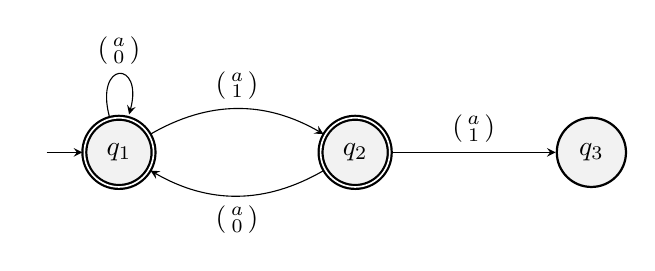
\begin{tikzpicture}
            \node[state, initial, accepting] (q1) {$q_1$};
            \node[state, accepting, right of=q1] (q2) {$q_2$};
            \node[state, right of=q2] (q3) {$q_3$};
            \draw (q1) edge[loop above] node{$\icol{a\\0}$} (q1)
            (q1) edge[bend left, above] node{$\icol{a\\1}$} (q2)
            (q2) edge[bend left, below] node{$\icol{a\\0}$} (q1)
            (q2) edge[above] node{$\icol{a\\1}$} (q3);
            \end{tikzpicture}
        \caption{Deterministic automaton recognizing the same language as expression $\varphi(X)$}
        \label{fig:my_label}
    \end{figure}
\end{example} \

The method we want to use to prove that 1Q sequences modulo are eventually periodic is to simplify 1Q expressions defining such sequences. The main complexity of 1Q expressions is usage of semiring quantifiers. To calculate values of sequence defined by expression like $\Sigma_X \ \varphi(X)$, it is necessary to know for how many valuations of $X$ the expressions $\varphi(X)$ is true, for words of length $1,2,\ldots$.

Fortunately, manipulations of automata corresponding to expressions with free variables like $\varphi(X)$ allow us to create nondeterministic automata that ``count'' the number of valuations for which $\varphi(X)$ is true.

\begin{lemma}
\label{LemElimVar}
    Let $\varphi$ be an MSO expression with a non-empty set of free variables $V = \{v_1, \ldots, v_n\}$. Let $A$ be its corresponding deterministic finite automaton, i.e. automaton recognizing the same language as $\varphi$. $\varphi$ and $A$ recognize language $L \subseteq \Sigma_V^*$. A word $(w, \sigma) \in L$ can equivalently be denoted in following way: $(w, \sigma(v_1), \ldots \sigma(v_n))$. Let $v_i \in V$. Define following language over reduced alphabet (by ``ignoring'' variable $v_i$): 
    $$L' = \{(w, \sigma(v_1), \ldots, \sigma(v_{i-1}), \sigma(v_{i+1}), \ldots, \sigma(v_n)) \ : \ (w, \sigma(v_1), \ldots \sigma(v_n)) \in L\}$$
    Now, following holds:
    \begin{enumerate}
        \item $L'$ can be recognized by automaton $A'$ identical to $A$, but defined over reduced alphabet $\Sigma_{V \setminus \{v_i\}} = \Sigma \times \{0, 1\}^{|V-1|}$. Transitions of $A'$ differ from transitions of $A$ by simply ignoring variable $v_i$,
        \item automaton $A'$ can turn nondeterministic and for arbitrary word
        $$w_{\setminus\{v_i\}} = (w, \sigma(v_1), \ldots, \sigma(v_{i-1}), \sigma(v_{i+1}), \ldots, \sigma(v_n)) \in L',$$ and 
        $$w^{-1}_{\setminus\{v_i\}} = \{(w, \sigma(v_1), \ldots, \sigma(v_{i-1}), x, \sigma(v_{i+1}), \ldots, \sigma(v_n)) \in L \ : \ x \in \{0, 1\}^* \},$$
        it is true that $nRuns_{A'}(w_{\setminus\{v_i\}}) = |w^{-1}_{\setminus\{v_i\}}|$. This means that the number of accepting runs of automaton $A'$ for some valuation of variables (ignoring removed variable $v_i$) corresponds to the number of accepting valuations of this variable with given valuation of remaining variables in original language $L$.
    \end{enumerate}
\end{lemma}

\begin{proof} \

    \begin{enumerate}
        \item $A'$ is simply an automaton recognizing projection of $\Sigma_V^*$ on $\Sigma_{V \setminus \{v_i\}}$ - ignoring one of the dimensions (corresponding to variable $v_i$).
        \item We can show that $A'$ can turn nondeterministic in following way. Let $\delta_A$ be the set of transitions of automaton $A$. Let $q_1, q_2, q_3 \in Q_A$ be some three states of automaton $A$ such that 
        $$q_1 \xrightarrow{(a, v_1, \ldots, v_{i-1}, 0, \ldots v_n)} q_2 \in \delta_A,$$ 
        $$q_1 \xrightarrow{(a, v_1, \ldots, v_{i-1}, 1, \ldots v_n)} q_3 \in \delta_A.$$
        From construction it follows that in $A'$ following situation happens:
        $$q_1 \xrightarrow{(a, v_1, \ldots, v_{i-1}, \ldots v_n)} q_2 \in \delta_{A'},$$ 
        $$q_1 \xrightarrow{(a, v_1, \ldots, v_{i-1}, \ldots v_n)} q_3 \in \delta_{A'},$$
        from which follows that $A'$ is nondeterministic. If there are no such states in $A$ then $A'$ remains deterministic. Now we have to prove that $nRuns_{A'}(w_{\setminus\{v_i\}}) = |w_L|$, for $w_{\setminus\{v_i\}} \in L'$. It follows directly from construction of $A'$, namely: to every accepting path of $w_{\setminus\{v_i\}}$ in automaton $A'$ corresponds some valuation of $v_i$, for which automaton $A$ must had accepted a word $(w, \sigma(v_1), \ldots, \sigma(v_{i-1}), \sigma(v_i), \sigma(v_{i+1}), \ldots, \sigma(v_n))$.
    \end{enumerate}
\end{proof}

\begin{example}[Fibonacci, continued]
\label{ExFibCont}
    Let us continue working on~\cref{ExFib}. There, we had following expression with a free variable $X$:
    $$\varphi(X) = \neg(\exists_{x_1}\exists_{x_2} \ x_1 \in X \land x_2 \in X \land x_2 > x_1 \land \neg(\exists_{x_3} \ x_3 > x_1 \land x_3 < x_2 ))$$
    We also constructed deterministic automaton recognizing language over extended alphabet $\Sigma_V = \{a\} \times \{0,1\}$. From~\cref{LemElimVar} we know that it's possible to build an automaton, possibly nondeterministic, that ignores one of the free variables and its number of runs corresponds to number of valuations of ignored variable. In this case, we achieve automaton presented in~\cref{fig:my_label2}.

    \begin{figure}[ht]
        \centering
        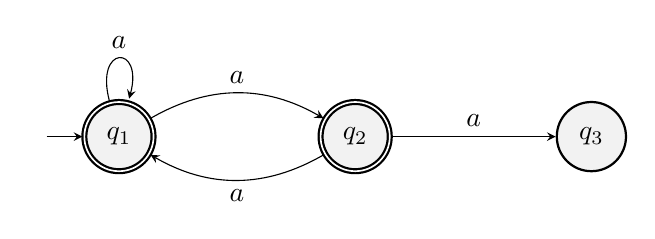
\begin{tikzpicture}
            \node[state, initial, accepting] (q1) {$q_1$};
            \node[state, accepting, right of=q1] (q2) {$q_2$};
            \node[state, right of=q2] (q3) {$q_3$};
            \draw (q1) edge[loop above] node{$a$} (q1)
            (q1) edge[bend left, above] node{$a$} (q2)
            (q2) edge[bend left, below] node{$a$} (q1)
            (q2) edge[above] node{$a$} (q3);
            \end{tikzpicture}
        \caption{Nondeterministic ``counting'' automaton that skips variable $X$ from $\varphi(X)$}
        \label{fig:my_label2}
    \end{figure}

    From explanation in~\cref{ExFib} of correspondence of $\varphi(X)$ and Fibonacci numbers, and from results in~\cref{LemElimVar} it should follow that the number of accepting runs of automaton shown in~\cref{fig:my_label2} for word of length $n$ ($a^n$) should equal $F(n+2)$. This is indeed true and can be proven by induction.
\end{example}

The following lemmas are crucial in semiring quantifiers elimination in 1Q expressions:

\begin{lemma}
    \label{QuantElimAdd}
    Let $\mathbb{Z}_m$ be a modulo semiring and $\varphi$ a simple recognizable step function on this semiring. Then $\Sigma_x \ \varphi$ and $\Sigma_X \ \varphi$ are also simple recognizable step functions.
\end{lemma}

\begin{proof}
    $\varphi$ is a simple recognizable step function, so it can be expressed as $\varphi = \sum_{i = 1}^{n} \ \varphi_{L_i} \cdot k_i$, where $\varphi_{L_i}$ are MSO expressions and $k_i \in \mathbb{Z}_m$. Now, consider the expression $\Sigma_{X} \ \varphi$, where $X$ is either a first-order or second-order variable. The reasoning is the same regardless of whether we work with first-order or second-order variables, so we will handle both simultaneously. Some of the MSO expressions inside $\varphi$ might contain $X$ as a free variable, while others might not. Nevertheless, in the semantics of QMSO, $\Sigma$ will iterate over all valuations of $X$ to evaluate this expression. We can assume that every MSO expression inside $\varphi$ contains $X$ as a free variable, by simply concatenating every expression with the always true expression $X = X$.

    Now, for every MSO expression $\varphi_{L_i}$ that appears inside $\varphi$, assign a deterministic finite automaton recognizing language $L_i$. These MSO expressions contain free variable $X$, so corresponding automata are defined over an extended alphabet. Having deterministic automata over extended alphabet we can use~\cref{LemElimVar} to build possibly nondeterministic ``counting'' automata. The number of runs of these automata corresponds to number of accepting valuations of free variable $X$.

    To handle addition - semiring quantifiers $\Sigma$ - it is only necessary to know how many times (modulo $m$) each constant $k_i$ appears. Count the number of runs (valuations) for automaton corresponding to $\varphi_{L_i}$ using~\cref{CountRunsAutomaton}. For every $\varphi_{L_i}$ and every $k < m$, create an automaton $\varphi_{L_i}^k$, accepting words over the reduced alphabet (i.e., ignoring variable $X$) for which the number of accepting valuations in the original automaton was equal to $k \mod m$. Now, addition quantifiers can be removed in following way:
    $$\Sigma_X \ \varphi = \sum_{i = 1}^n \sum_{j = 0}^{m-1} \ \varphi_{L_i}^j \cdot (j \cdot k_i \mod m).$$
    $\varphi_{L_i}^j$ can be true for at most one $j$, $0 \leq j \leq m-1$. This $j$ marks the number of successful runs modulo $m$, that is, the number of valuations of $X$ for which $\varphi_{L_i}$ was true. In the original expression, we would add $k_i$ for each such valuation, giving us $j \cdot k_i$ for this part of the expression. Since we work modulo $m$, every such value is taken modulo $m$.
\end{proof}

\begin{lemma}
    \label{QuantElimMult}
    Let $\mathbb{Z}_m$ be a modulo semiring and $\varphi$ a simple recognizable step function on this semiring. Then $\Pi_x \ \varphi$ and $\Pi_X \ \varphi$ are also simple recognizable step functions.
\end{lemma}

\begin{proof}
    $\varphi$ is a simple recognizable step function, so it can be expressed as $\varphi = \sum_{i = 1}^{n} \ \varphi_{L_i} \cdot k_i$, where $\varphi_{L_i}$ are MSO expressions and $k_i \in \mathbb{Z}_m$. Proof for this lemma will use similar reasoning to that in~\cref{QuantElimAdd}, but with additional complexity. Once again, we need to determine how many times each constant $k_i$ appears across all valuations of variable bound by quantifier. However, it is insufficient to know how many times this constant appears modulo $m$, as in the case of exponentiation modulo, different numbers have different periods. For example, consider constant $2$ when working modulo $3$. We have $2^1 \mod 3 = 2$, $2^2 \mod 3 = 1$, $2^3 \mod 3 = 2$, and so on. For odd exponents, the value will always be $2$, and for even exponents, it will be $1$. Therefore, in this case, we need to know the number of valuations modulo $2$, not $3$. 

    It is also different for constants that are roots of any order of $m$. Suppose we work modulo $m = 16$ and we have a constant $k_i = 2$. Now, $2^1 \mod 16 = 2$, $2^2 \mod 16 = 4$, $2^3 \mod 16 = 8$, $2^4 \mod 16 = 0$, $2^5 \mod 16 = 0$, and so on. Thus, after reaching $2^4$, for all subsequent exponents, the value will be $0$. In this case we have a prefix sequence $2,4,8$, followed by a constant sequence of $0$.

    General case is following. Consider a constant $k_i$, which we exponentiate modulo $m$. The sequence $Exp_{k_i} = (k_i)^1 \mod m, (k_i)^2 \mod m, (k_i)^3 \mod m \ldots$ is eventually periodic, which follows from the fact that this sequence can achieve at most $m$ different values, and $(k_i)^{n_i} \mod m = (k_j)^{n_j} \mod m \implies (k_i)^{n_i + 1} \mod m = (k_j)^{n_j + 1} \mod m$ (i.e. after reaching a cycle, it is not possible to escape it). As this sequence is eventually periodic, there exists $N_i, p_i \in \mathbb{N}$, $p_i > 0$ such that $\forall_{n > N_i} \ Exp_{k_i}(n) = Exp_{k_i}(n + p_i)$. So there is a prefix of length $N_i$ (empty for $N_i = 0$), and then a repeating cycle of length $p_i$. 

    To know what is the influence of constant $k_i$ on the whole expression, we need to introduce $N_i + p_i$ new constants and MSO expressions. First, for $0 < j \leq N_i$, introduce constant $k_i^j = (k_i)^j \mod m$ and MSO expression $\varphi_{L_i}^j$ that expresses that there exist exactly $j$ different valuations of $X$ for which $\varphi_{L_i}$ is true, i.e. $\varphi_{L_i}^j = \exists^{=j} \ \varphi_{L_i}$. This handles prefix of length $N_i$. Next, for $N_i < j \leq N_i + p_i$ introduce constant $k_i^j = (k_i)^j \mod m$ and a MSO expression $\varphi_{L_i}^j$ expressing that there exist more than $N_i$ different valuations of $X$ for which $\varphi_{L_i}$ is true and this number of valuations is equal to $j \mod p_i$. For second property use automaton counting number of runs modulo from~\cref{CountRunsAutomaton}, the same way we did in addition case~\cref{QuantElimAdd}.

    We also need to handle special case when constant $k_i$ has no influence on the whole expression, that is: $\varphi_{L_i}$ is false for every valuation of $X$. To handle this case introduce $k_i^j = 1$ (neutral element of multiplication) and $\varphi_{L_i}^j = \neg(\exists_X \ \varphi_{L_i})$.

    From what we have, the value corresponding to some $k_i$ of the original expression, after quantifier elimination, is $\sum_{j = 0}^{N_i + p_i} \ (\varphi_{L_i}^j \cdot k_i^j)$. The inner MSO expression $\varphi_{L_i}^j$ will be true for exactly one $j$.
    
    Now, multiplication quantifiers can be removed in following way:
    $$\Pi_X \ \varphi = \prod_{i = 1}^n \ \sum_{j = 0}^{N_i + p_i} \ \varphi_{L_i}^j \cdot k_i^j.$$
\end{proof}

Finally, we can characterize 1Q sequences on a modulo semiring as simple recognizable step functions:

\begin{lemma}
    \label{OverModAreSimpleRec}
    Let $\mathbb{Z}_m$ be a modulo semiring and $\varphi$ be a 1Q sentence over $\mathbb{Z}_m$. Then a sequence defined by $\varphi$ can be defined as a simple recognizable step function (i.e. $\varphi$ can be reduced to a form of simple recognizable step function). 
\end{lemma}

\begin{proof}
    We use induction on the structure of expression $\varphi$. For base case - expressions without quantification at the semiring level - it follows from~\cref{QFreeRecognizable} and~\cref{RecEqSimpleRec}. 
    
    Sum and product of two simple recognizable step functions is a simple recognizable step function - it follows from induction step of proof of~\cref{DefRecStepFun} and from~\cref{RecEqSimpleRec}.

    Consider an expression $\varphi = Q_Y \ \theta$, where $\theta$ is a simple recognizable step function, $Q$ a semiring quantifier and $Y$ first order or second order variable. By lemmas~\ref{QuantElimAdd} and~\ref{QuantElimMult} it follows that $\varphi$ is a simple recognizable step function. This finishes the proof.
\end{proof}

\begin{fact}
    \label{InvAreReg}
    Let $S$ be a power series definable by a simple recognizable step function $S = \sum_{i = 1}^{n} \ \varphi_{L_i} \cdot k_i$. Language of words for which $S$ achieves value $k_i$ is exactly $\varphi_{L_i}$ (which is a regular language).
\end{fact}

\begin{proof}
    This follows directly from definition of simple recognizable step function and the fact that $\varphi_{L_i}$ is a MSO expression.
\end{proof}

From these results, an important characterization of 1Q sequences on modulo semirings follows: 1Q sequences on modulo semirings are eventually periodic.

\begin{lemma}
    \label{OverModAreSimpleRec2}
    Let $\mathbb{Z}_m$ be a modulo semiring and $\varphi$ be a 1Q sentence over $\mathbb{Z}_m$. Then a sequence defined by $\varphi$ is eventually periodic.
\end{lemma}

\begin{proof}
    Thanks to~\cref{OverModAreSimpleRec} we know that $\varphi$ reduces to simple recognizable step function. Additionaly, by~\cref{InvAreReg}, we know that language of words for which sequence defined by $\varphi$ achieves a given value $k_i$ is a regular language. There is a finite number of values this sequence can achieve (at most $m$). Regular languages on one-letter alphabets are eventually periodic with regard to word length (\cite[Theorem 1]{PighizziniS02}).

    There are $m$ regular, disjoint languages $L_1, \ldots, L_m$ corresponding to different constants $k_i$. We assume these languages don't accept empty word. Each language $L_i$ is eventually periodic with regard to word length, so there exist $N_i, p_i \in \mathbb{N}$, such that $\forall_{n \geq N_i} \ a^n \in L_i \iff a^{n + p} \in L_i$. To find a ``global'' period that works for all langauges, take $N = \prod_{i=1}^m \ N_i$, $p = \prod_{i=1}^m \ p_i$. This period is simultaneously a period for every $L_i$ since $N$ divides each $N_i$ and $p$ divides each $p_i$.
\end{proof}

From this, the main result of this section,~\cref{1QSequencesPeriodic}, directly follows:

\begin{proof}[Proof of~\cref{1QSequencesPeriodic}]
    1Q sequences modulo are the same as 1Q sequences over a modulo semiring (\cref{1QModulo}). The result then follows directly from~\cref{OverModAreSimpleRec2}.
\end{proof}

\begin{corollary}
    Catalan numbers are not 1Q-definable
\end{corollary}

\begin{proof}
    The reasoning is the same as in~\cite[Theorem 7, Corollary 8]{CadilhacMPPS20}, which uses results about Catalan sequences from~\cite{KubotaCatalan} - Catalan numbers are not ultimately periodic modulo prime numbers $p > 3$, while 1Q-definable sequences are. Therefore, Catalan numbers are not 1Q-definable.
\end{proof}

\section{Other subjects}
While researching 1Q sequences, there were other interesting subjects to go into, but were not completed.

\subsection*{Characterization of 1Q sequences}
1Q expressions allow to define wide class of sequences. In particular, whole class of linear recursive sequences is contained in 1Q sequences. The interesting research question is exactly what class of sequences is defined by 1Q expressions - if there is other, maybe simpler representation of such sequences?

In Introduction it was mentioned that 1Q expressions allow defining a sequence that is not polynomial recursive. From this follows interesting question: is every polynomial recursive sequence also 1Q-definable? It does not seem easy to answer, as it is not trivial to express recursion with 1Q expressions.

\subsection*{Complexity of zero checking}
Suppose we work over modulo semiring. What is the time complexity with regard to length of sentence $\varphi$ of checking whether sequence defined by such a sentence is constantly equal $0$? 

Lower bound for this problem (i.e. how far can the first non-zero element be) is at least TOWER. This follows from the fact that...

\subsection*{1Q on first order logic}
It might be interesting to look into following restriction of 1Q expressions: we can only use first order variables on semiring level and logical level (i.e. we move from MSO logic to FO logic). 

First, let's focus on behavior of these sequences modulo.

As stated in Droste paper, first order definable series coincide with series definable by weighted automata when working with aperiodic semirings. Unfortunately, semirings we're working with - semirings for modulo operations - aren't aperiodic. It can be easily with sequence defined by following expression:

$$ \Sigma_x \ . \ 1 $$

It defines the following sequence modulo 2: $\{1, 0, 1, 0, 1, \ldots\}$, which is not aperiodic. What's even more interesting is that inverse images of values of this sequence are not FO-definable languages. For value $0$ inverse image is a language of words of even length, which is only definable in second order logic. 

We might want to ask if it's possible to define following sequence in 1Q modulo 2 using FOL: $\{0, 0, 1, 0, 0, 1, \ldots\}$, that is: we have ones on positions divisible by 3. 

\bibliographystyle{plainurl}
\bibliography{bib}

\end{document}
